\chapter{Arhitektura i dizajn sustava}

		Glavni prioriteti kod izgradnje sustava i odabira arhitekture su nam jednostavnost korištenja sučelja za sve korisnike(osobito za građane), paralelni rad više korisnika u stvarnom vremenu te korištenje na različitim uređajima(prvenstveno na mobilnim). Osim toga, građani najvjerojatnije neće biti voljni instalirati dodatnu programsku podršku, već će se htjeti koristiti onim što već imaju, a to je standardni web preglednik. Zbog navedenih zahtjeva, odlučili smo se za arhitekturu responzivne web aplikacije.
		\newline
		
		\textbf{Arhitekturu} možemo podijeliti na tri osnovna podsustava:
		\begin{packed_item}
		\item Web poslužitelj
		\item Web aplikacija
		\item Baza podataka
		\end{packed_item}
		
		\begin{figure}[H]
					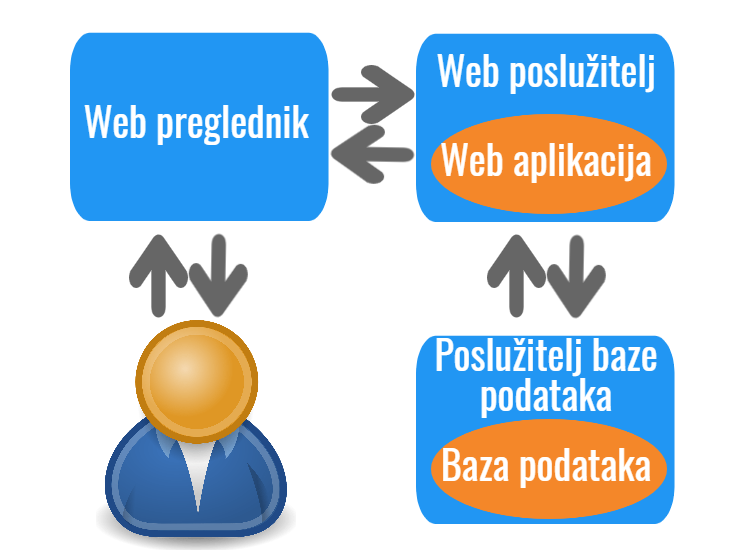
\includegraphics[scale=0.6]{slike/webapp.png}
					\centering
					\caption{Arhitektura sustava}
					\label{fig:Arhitektura-sustava}
		\end{figure}
		\newpage
		
		\textbf{Web preglednik} je program koji omogućuje korisnicima pregled web-stranica i sadržaja vezanih uz njih. Web preglednici su prevoditelji, tj. stranice su pisane u kodu koji preglednici nakon toga interpretiraju u nešto razumljivo. Korisnik putem web preglednika šalje zahtjev web poslužitelju.
		
		\textbf{Web poslužitelj} je osnova rada web aplikacije. Glavna mu je zadaća komunikacija klijenta s aplikacijom. Komunikacija se vrši putem HTTP (engl. Hyper Text Transfer Protocol) protokola,  glavne i najčešće metode prijenosa informacija na Webu.  Osnovna namjena ovog protokola je omogućavanje objavljivanja i prezentacije HTML dokumenata, tj. web stranica. Poslužitelj pokreće web aplikaciju te joj prosljeđuje zahtjev.
		
        Korisnik koristi \textbf{web aplikaciju} za obrađivanje željenih zahtijeva. Web aplikacija obrađuje zahtjev, pristupa bazi podataka te preko poslužitelja vraća korisniku odgovor u obliku HTML dokumenta vidljivog u web pregledniku.
        
        Programski jezici koje smo odabrali za izradu naše web aplikacije su Java zajedno sa Spring Boot radnim okvirom za izradu backenda 
        te React i jezik Javascript za izradu frontenda.
        \newline
        
        Arhitektura sustava razvijat će se prema \textbf{MVC} (Model-View-Controller) konceptu. 
        MVC odvaja korisničko sučelje od ostatka sustava, pogodan je za uporabu razinske kohezije te smanjuje međuovisnost između U/I sučelja i ostatka sustava. Posljedica toga je jednostavnije ispitivanje i razvijanje i dodavanje novih svojstava u sustav.
        \newline
        
        MVC se sastoji od: 
        
        \begin{packed_item}
		\item \textbf{Model}
		\item \textbf{View}
		\item \textbf{Controller}
		\end{packed_item}
		
		\begin{figure}[H]
					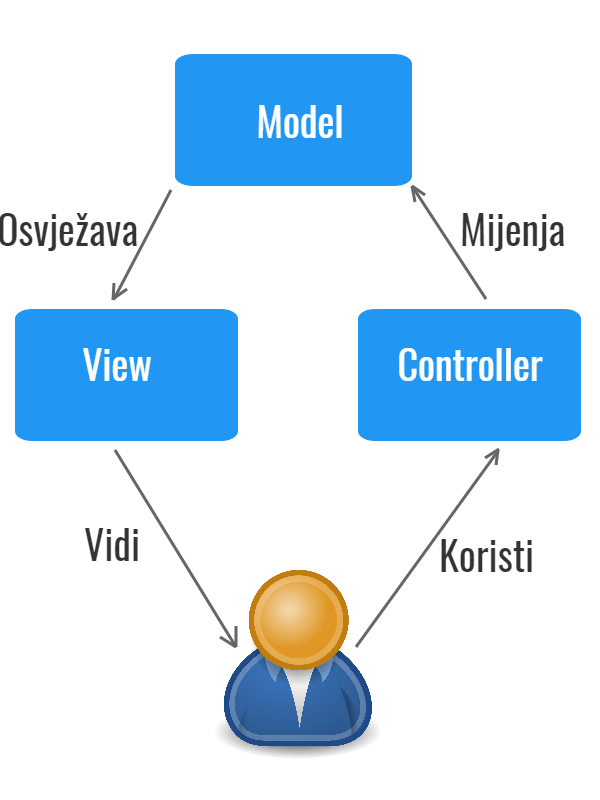
\includegraphics[scale=0.6]{slike/mvcskica.png}
					\centering
					\caption{MVC skica}
					\label{fig:MVC-skica}
		\end{figure}
		
		
		Model čuva podatke web aplikacije, logiku i pravila aplikacije te je centralna komponenta sustava. 
		
		Controller prima ulaze i prilagođava ih za prosljeđivanje Modelu ili Viewu. Nadalje, upravlja korisničkim zahtjevima te pomoću njih izvodi daljnju komunikaciju i interakciju s ostalim elementima sustava. 
		
		View predstavlja bilo kakav prikaz podataka te su mogući različiti prikazi istih. 
		
		Korisnik koristi Controller te vidi View. Controller mijenja Model, a model osvježava View.
		\newpage
        
			
		\section{Baza podataka}
		
		
		Aplikacija koristi SQL relacijsku bazu podataka. Ona se sastoji od relacija (tablica) koje se sastoje od atributa. Razlog uporabe relacijske baze podataka je olakšavanje modeliranja entiteta i događaja iz stvarnog svijeta. Baza podataka ove aplikacije sastoji se od sljedećih entiteta:
		
		\begin{packed_item}
			
			\item Korisnik
			\item Kontejner
			\item Komunalna služba
			\item Pretplata
			\item Recenzija
			\item Senzor
			\item Zona
			\item Grad
			\item Država
			
		\end{packed_item}
		
			\subsection{Opis tablica}
				
				\textbf{Korisnik.} Ovaj entitet sadrži informacije o korisniku aplikacije. Uključeni atributi su ID korisnika, ID komunalne službe u kojoj je korisnik zaposlen (ako je zaposlen u komunalnoj službi), korisničko ime, e-mail adresa, informacije je li e-mail adresa potvrđena te lozinka. Ovaj entitet u vezi je \textit{One-to-Many} s entitetom Komunalna služba preko ID-a korisnika te u vezi \textit{Many-to-One} s entitetom Komunalna služba preko ID-a komunalne službe u kojoj je korisnik zaposlen.
				
				\begin{longtabu} to \textwidth {|X[6, l]|X[6, l]|X[20, l]|}
					
					\hline \multicolumn{3}{|c|}{\textbf{Korisnik}}\\[3pt] \hline
					\endfirsthead
					
					\hline \multicolumn{3}{|c|}{\textbf{Korisnik}}\\[3pt] \hline
					\endhead
					
					\hline 
					\endlastfoot
					
					\cellcolor{LightGreen}IDkorisnik & INTEGER & Jedinstveni identifikator korisnika\\ \hline
					\cellcolor{LightBlue}IDsluzba & INTEGER & Jedinstveni identifikator komunalne službe\\ \hline 
					korisnickoIme & VARCHAR & Korisničko ime\\ \hline 
					email & VARCHAR & E-mail adresa korisnika\\ \hline 
					emailPotvrda & BOOLEAN & Stanje potvrđenosti e-mail adrese\\ \hline 
					lozinka & VARCHAR & Hash lozinke\\ \hline 
					
				\end{longtabu}
			
				\textbf{Kontejner.} Ovaj entitet sadrži informacije o kontejneru. Uključeni atributi su ID kontejnera, ID komunalne službe, ID zone u kojoj se kontejner nalazi, adresa kontejnera, geografska dužina te geografska širina kontejnera. Ovaj entitet u vezi je \textit{One-to-Many} s entitetom Pretplata, Recenzija i Senzor preko ID-a kontejnera, \textit{Many-to-One} s entitetom Komunalna služba preko ID-a komunalne službe te u vezi \textit{Many-to-One} s entitetom Zona preko ID-a zone.
				
				\begin{longtabu} to \textwidth {|X[6, l]|X[6, l]|X[20, l]|}
					
					\hline \multicolumn{3}{|c|}{\textbf{Kontejner}}\\[3pt] \hline
					\endfirsthead
					
					\hline \multicolumn{3}{|c|}{\textbf{Kontejner}}\\[3pt] \hline
					\endhead
					
					\hline 
					\endlastfoot
					
					\cellcolor{LightGreen}IDkontejner & INTEGER & Jedinstveni identifikator kontejnera\\ \hline
					\cellcolor{LightBlue}IDsluzba & INTEGER & Jedinstveni identifikator komunalne službe\\ \hline 
					\cellcolor{LightBlue}IDzona & INTEGER & Jedinstveni identifikator gradske zone\\ \hline 
					adresa & VARCHAR & Adresa kontejnera\\ \hline 
					geoDuzina & NUMERIC & Geografska dužina kontejnera\\ \hline 
					geoSirina & NUMERIC & Geografska širina kontejnera\\ \hline 
					
				\end{longtabu}
			
				\textbf{Komunalna služba.} Ovaj entitet sadrži informacije o komunalnoj službi. Uključeni atributi su ID komunalne službe, ID direktora komunalne službe, ime komunalne službe te opis komunalne službe. Ovaj entitet u vezi je \textit{One-to-Many} s entitetom Korisnik i Kontejner preko ID-a komunalne službe te u vezi \textit{Many-to-One} s entitetom Korisnik preko ID-a direktora komunalne službe.
				
				\begin{longtabu} to \textwidth {|X[6, l]|X[6, l]|X[20, l]|}
					
					\hline \multicolumn{3}{|c|}{\textbf{Komunalna služba}}\\[3pt] \hline
					\endfirsthead
					
					\hline \multicolumn{3}{|c|}{\textbf{Komunalna služba}}\\[3pt] \hline
					\endhead
					
					\hline 
					\endlastfoot
					
					\cellcolor{LightGreen}IDsluzba & INTEGER & Jedinstveni identifikator komunalne službe\\ \hline
					\cellcolor{LightBlue}IDdirektor & INTEGER & Jedinstveni identifikator direktora komunalne službe\\ \hline 
					imeSluzba & VARCHAR & Ime komunalne službe\\ \hline 
					opisSluzba & VARCHAR & Opis komunalne službe\\ \hline
					
				\end{longtabu}
			
				\textbf{Pretplata.} Ovaj entitet sadrži informacije o korisničkim pretplatama na kontejnere. Uključeni atributi su ID korisnika i ID kontejnera. Ovaj entitet u vezi je \textit{Many-to-One} s entitetom Korisnik preko ID-a korisnika te u vezi \textit{Many-to-One} s entitetom Kontejner preko ID-a kontejnera.
				
				\begin{longtabu} to \textwidth {|X[6, l]|X[6, l]|X[20, l]|}
					
					\hline \multicolumn{3}{|c|}{\textbf{Pretplata}}\\[3pt] \hline
					\endfirsthead
					
					\hline \multicolumn{3}{|c|}{\textbf{Pretplata}}\\[3pt] \hline
					\endhead
					
					\hline 
					\endlastfoot
					
					\cellcolor{LightGreen}IDkorisnik & INTEGER & Jedinstveni identifikator komunalne službe\\ \hline
					\cellcolor{LightGreen}IDkontejner & INTEGER & Jedinstveni identifikator direktora komunalne službe\\ \hline 
					
				\end{longtabu}
			
				\textbf{Recenzija.} Ovaj entitet sadrži informacije o recenzijama kontejnera. Uključeni atributi su ID recenzije, ID korisnika, ID kontejnera, ocjena punoće, ocjena urednosti, komentar, slika te vrijeme objave recenzije. Ovaj entitet u vezi je \textit{Many-to-One} s entitetom Korisnik preko ID-a korisnika te u vezi \textit{Many-to-One} s entitetom Kontejner preko ID-a kontejnera.
				
				\begin{longtabu} to \textwidth {|X[6, l]|X[6, l]|X[20, l]|}
					
					\hline \multicolumn{3}{|c|}{\textbf{Recenzija}}\\[3pt] \hline
					\endfirsthead
					
					\hline \multicolumn{3}{|c|}{\textbf{Recenzija}}\\[3pt] \hline
					\endhead
					
					\hline 
					\endlastfoot
					
					\cellcolor{LightGreen}IDrecenzija & INTEGER & Jedinstveni identifikator recenzije\\ \hline
					\cellcolor{LightBlue}IDkorisnik & INTEGER & Jedinstveni identifikator korisnika\\ \hline 
					\cellcolor{LightBlue}IDkontejner & INTEGER & Jedinstveni identifikator kontejnera\\ \hline 
					ocjenaPunoce & INTEGER & Ocjena punoće kontejnera\\ \hline
					ocjenaUrednosti & INTEGER & Ocjena urednosti kontejnera\\ \hline
					komentar & VARCHAR & Komentar na stanje kontejnera u trenutku objavljivanja recenzije\\ \hline
					slika & LONGBLOB & Slika kontejnera u trenutku objavljivanja recenzije\\ \hline
					vrijemeObjave & TIMESTAMP & Vrijeme u trenutku objavljivanja recenzije\\ \hline
					
				\end{longtabu}
			
				\textbf{Senzor.} Ovaj entitet sadrži informacije o senzoru. Uključeni atributi su ID senzora, ID kontejnera te token. Ovaj entitet u vezi je \textit{Many-to-One} s entitetom Kontejner preko ID-a kontejnera.
				
				\begin{longtabu} to \textwidth {|X[6, l]|X[6, l]|X[20, l]|}
					
					\hline \multicolumn{3}{|c|}{\textbf{Senzor}}\\[3pt] \hline
					\endfirsthead
					
					\hline \multicolumn{3}{|c|}{\textbf{Senzor}}\\[3pt] \hline
					\endhead
					
					\hline 
					\endlastfoot
					
					\cellcolor{LightGreen}IDsenzor & INTEGER & Jedinstveni identifikator senzora\\ \hline
					\cellcolor{LightBlue}IDkontejner & INTEGER & Jedinstveni identifikator kontejnera\\ \hline 
					token & VARCHAR & Token senzora\\ \hline
					
				\end{longtabu}
			
				\textbf{Zona.} Ovaj entitet sadrži informacije o gradskoj zoni u kojoj je smješten kontejner. Uključeni atributi su ID zone, ID grada te ime zone. Ovaj entitet u vezi je \textit{One-to-Many} s entitetom Kontejner preko ID-a zone te u vezi \textit{Many-to-One} s entitetom Grad preko ID-a grada.
				
				\begin{longtabu} to \textwidth {|X[6, l]|X[6, l]|X[20, l]|}
					
					\hline \multicolumn{3}{|c|}{\textbf{Zona}}\\[3pt] \hline
					\endfirsthead
					
					\hline \multicolumn{3}{|c|}{\textbf{Zona}}\\[3pt] \hline
					\endhead
					
					\hline 
					\endlastfoot
					
					\cellcolor{LightGreen}IDzona & INTEGER & Jedinstveni identifikator gradske zone\\ \hline
					\cellcolor{LightBlue}IDgrad & INTEGER & Jedinstveni identifikator grada\\ \hline 
					imeZona & VARCHAR & Ime zone\\ \hline
					
				\end{longtabu}
			
				\textbf{Grad.} Ovaj entitet sadrži informacije o gradu u kojoj je smješten kontejner. Uključeni atributi su ID grada, ID države te ime grada. Ovaj entitet u vezi je \textit{One-to-Many} s entitetom Zona preko ID-a grada te u vezi \textit{Many-to-One} s entitetom Država preko ID-a države.
				
				\begin{longtabu} to \textwidth {|X[6, l]|X[6, l]|X[20, l]|}
					
					\hline \multicolumn{3}{|c|}{\textbf{Grad}}\\[3pt] \hline
					\endfirsthead
					
					\hline \multicolumn{3}{|c|}{\textbf{Grad}}\\[3pt] \hline
					\endhead
					
					\hline 
					\endlastfoot
					
					\cellcolor{LightGreen}IDgrad & INTEGER & Jedinstveni identifikator grada\\ \hline
					\cellcolor{LightBlue}IDdrzava & INTEGER & Jedinstveni identifikator države\\ \hline 
					imeGrad & VARCHAR & Ime grada\\ \hline
					
				\end{longtabu}
			
				\textbf{Država.} Ovaj entitet sadrži informacije o državi u kojoj je smješten kontejner. Uključeni atributi su ID države te ime države. Ovaj entitet u vezi je \textit{One-to-Many} s entitetom Grad preko ID-a države.
				
				\begin{longtabu} to \textwidth {|X[6, l]|X[6, l]|X[20, l]|}
					
					\hline \multicolumn{3}{|c|}{\textbf{Država}}\\[3pt] \hline
					\endfirsthead
					
					\hline \multicolumn{3}{|c|}{\textbf{Države}}\\[3pt] \hline
					\endhead
					
					\hline 
					\endlastfoot
					
					\cellcolor{LightGreen}IDdrzava & INTEGER & Jedinstveni identifikator države\\ \hline
					imeDrzava & VARCHAR & Ime države\\ \hline
					
				\end{longtabu}
			
			
			
			
			\subsection{Dijagram baze podataka}
				\begin{figure}[H]
					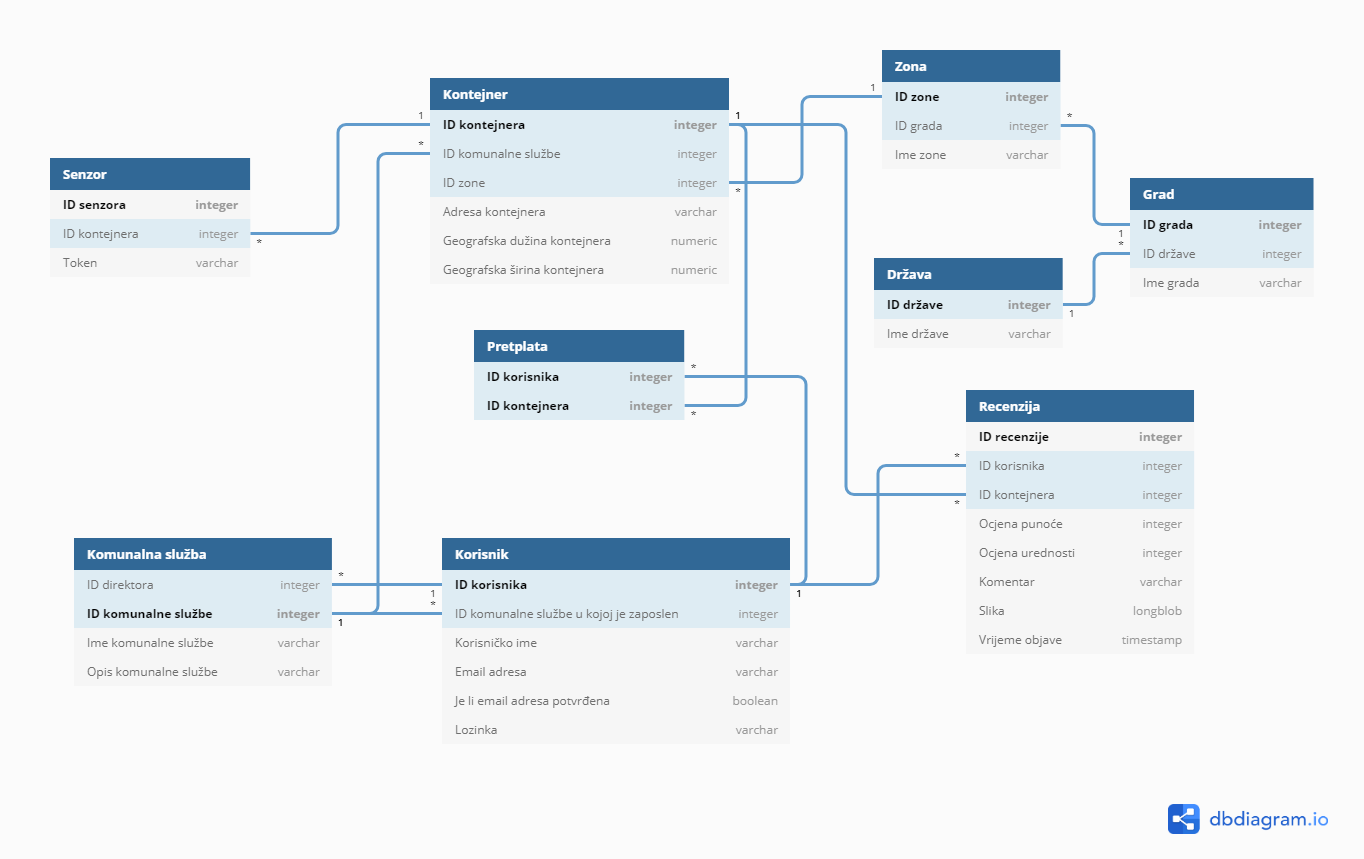
\includegraphics[width=1.0\linewidth]{slike/dijagramBaze.png}
					\centering
					\caption{Dijagram baze podataka}
					\label{fig:promjene}
				\end{figure}
			
			Dijagram baze podataka je izrađen alatom \href{https://dbdiagram.io}{dbdiagram.io}. Svjetlo plavo su označeni strani ključevi, a primarni ključevi su podebljani. 
			
			\eject
			
			
		\section{Dijagram razreda}
		
			Na slikama \ref{fig:controllers}, \ref{fig:DTO} i \ref{fig:models} su prikazani razredi \textit{backenda}.
			Razredi su podijeljeni u dijagrame prema njihovim odgovornostima: controller razredi odgovaraju na upite \textit{frontenda} te koriste razrede models za komunikaciju s bazom podataka i razrede DTO \engl{Data Transfer Object} za komunikaciju s \textit{frontendom} u JSON formatu.
			Radi preglednosti na dijagramima razreda su prikazane samo veze između razreda prikazanih na istom dijagramu.
		
			
			\begin{figure}[H]
				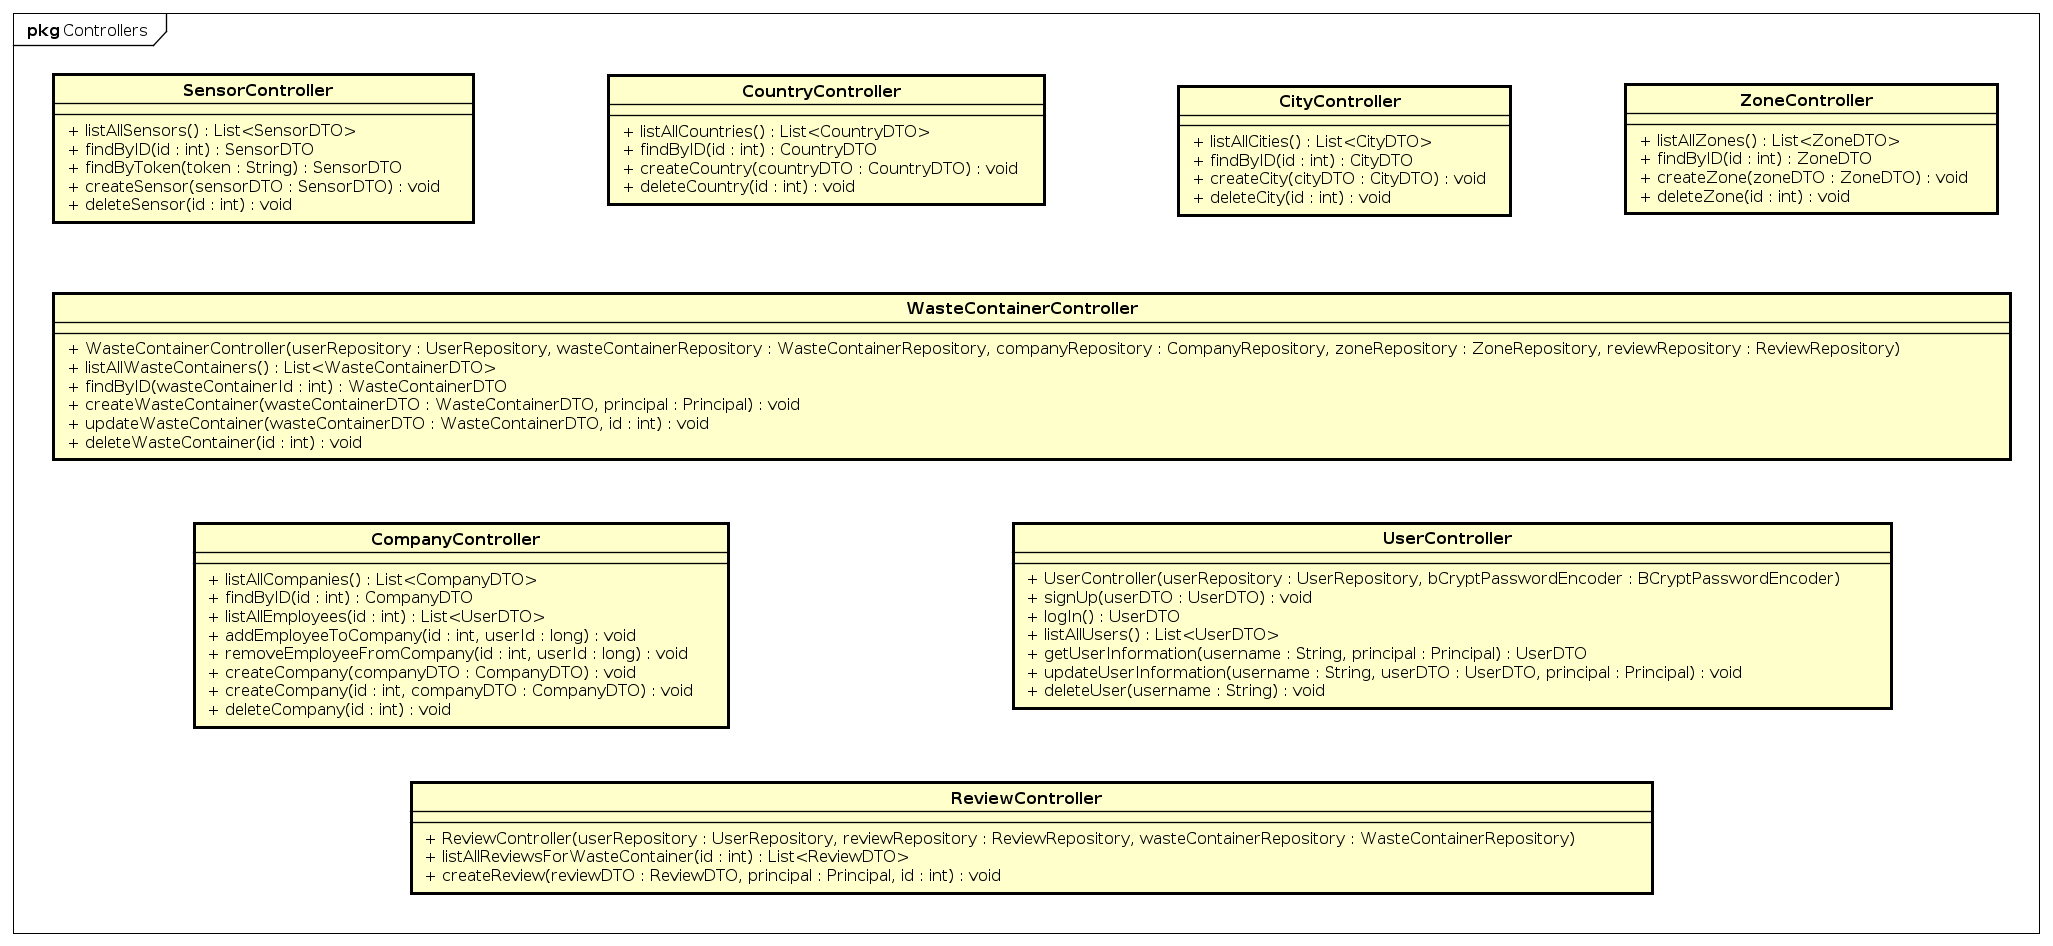
\includegraphics[width=1.0\linewidth]{slike/Controllers.png}
				\centering
				\caption{Dijagram razreda - dio Controllers}
				\label{fig:controllers}
			\end{figure}
		
			
			\begin{figure}[H]
				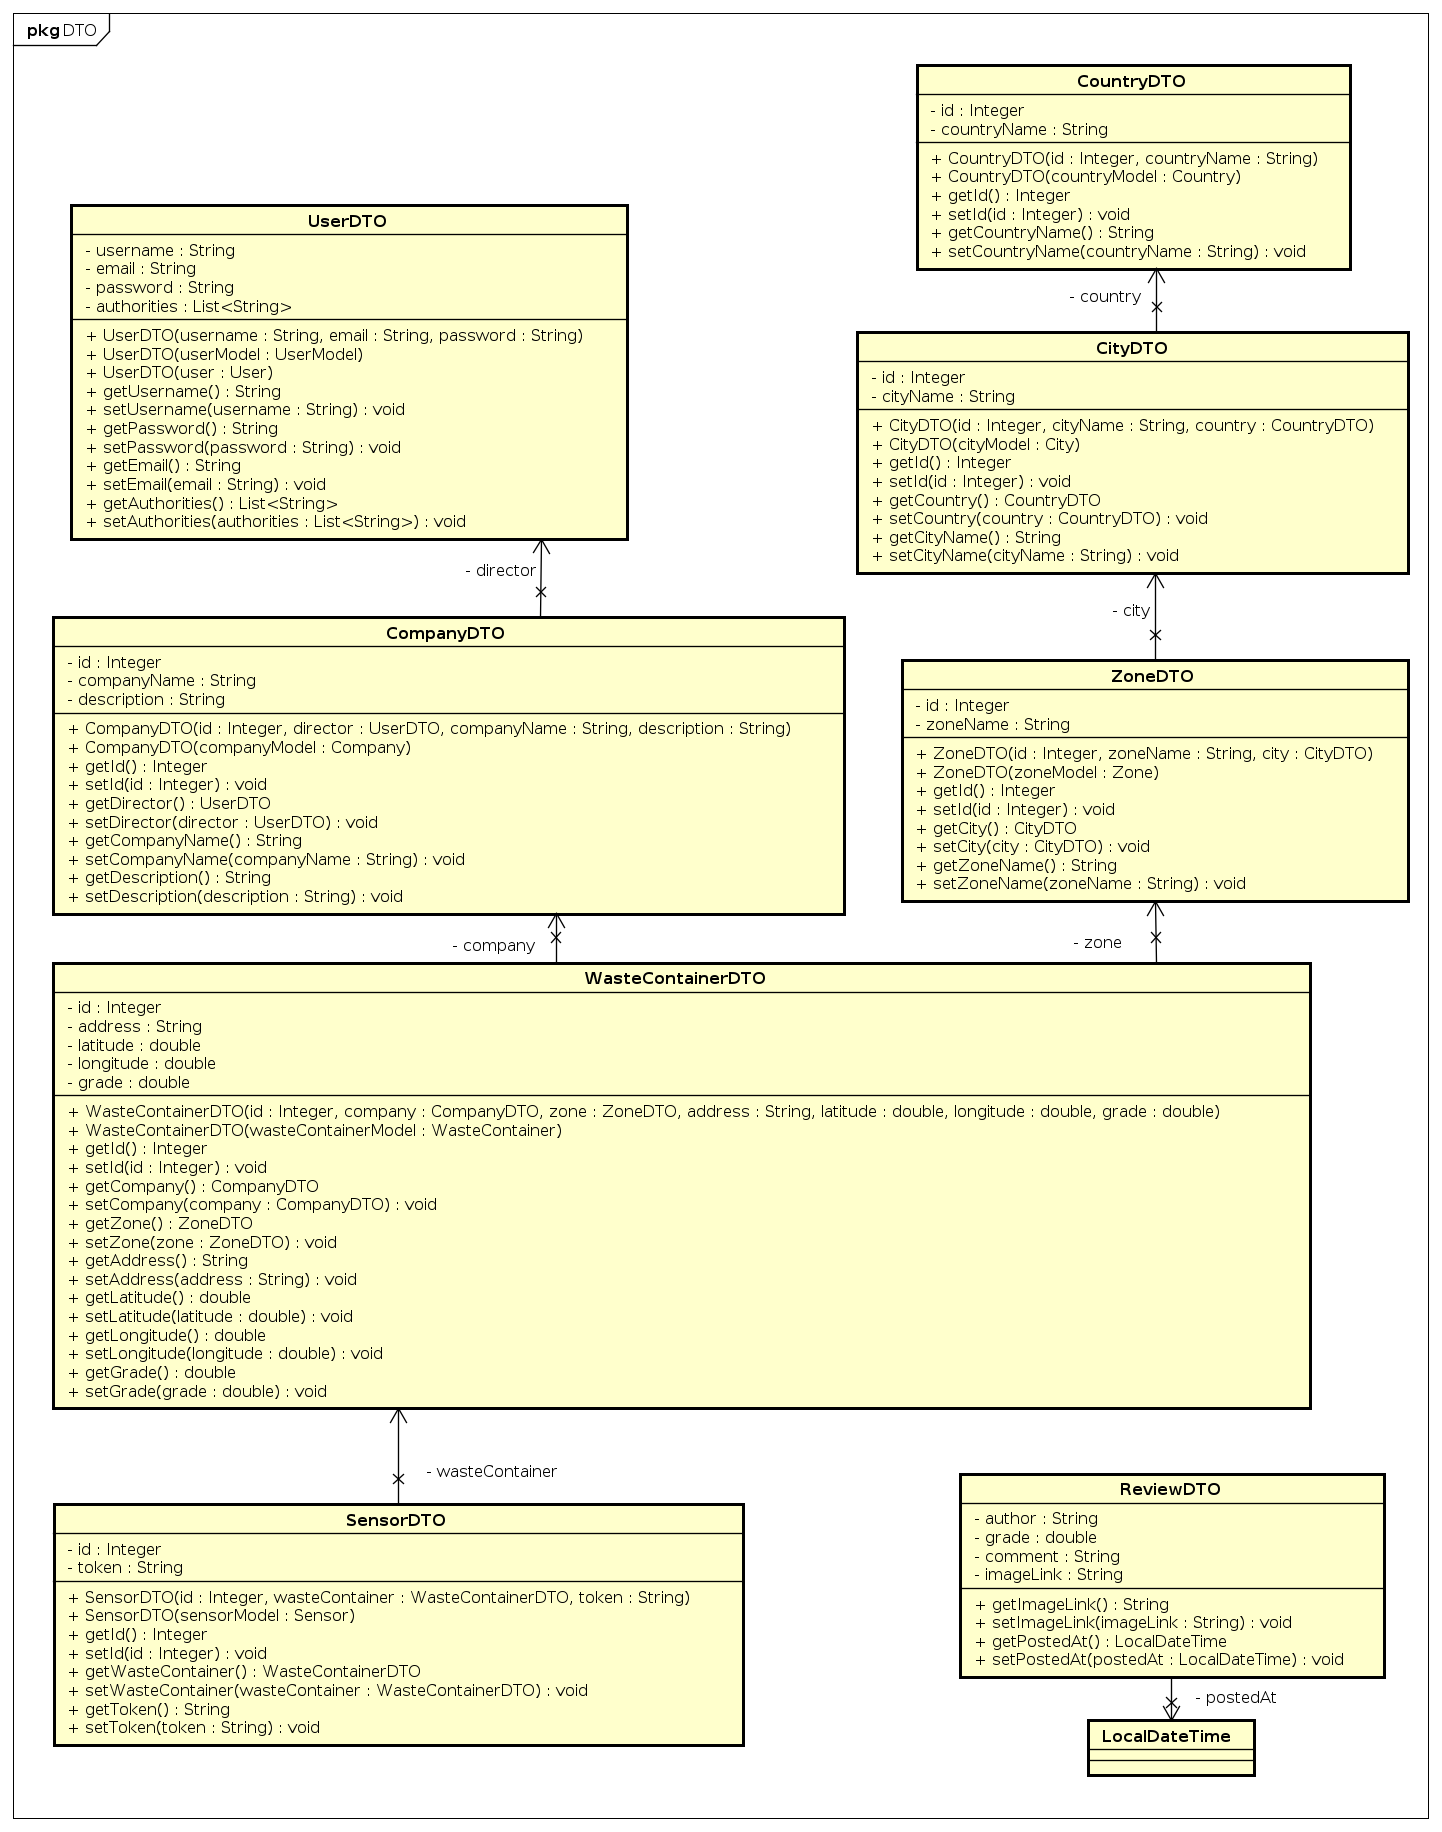
\includegraphics[width=1.0\linewidth]{slike/DTO.png}
				\centering
				\caption{Dijagram razreda - dio DTO}
				\label{fig:DTO}
			\end{figure}

			\begin{figure}[H]
				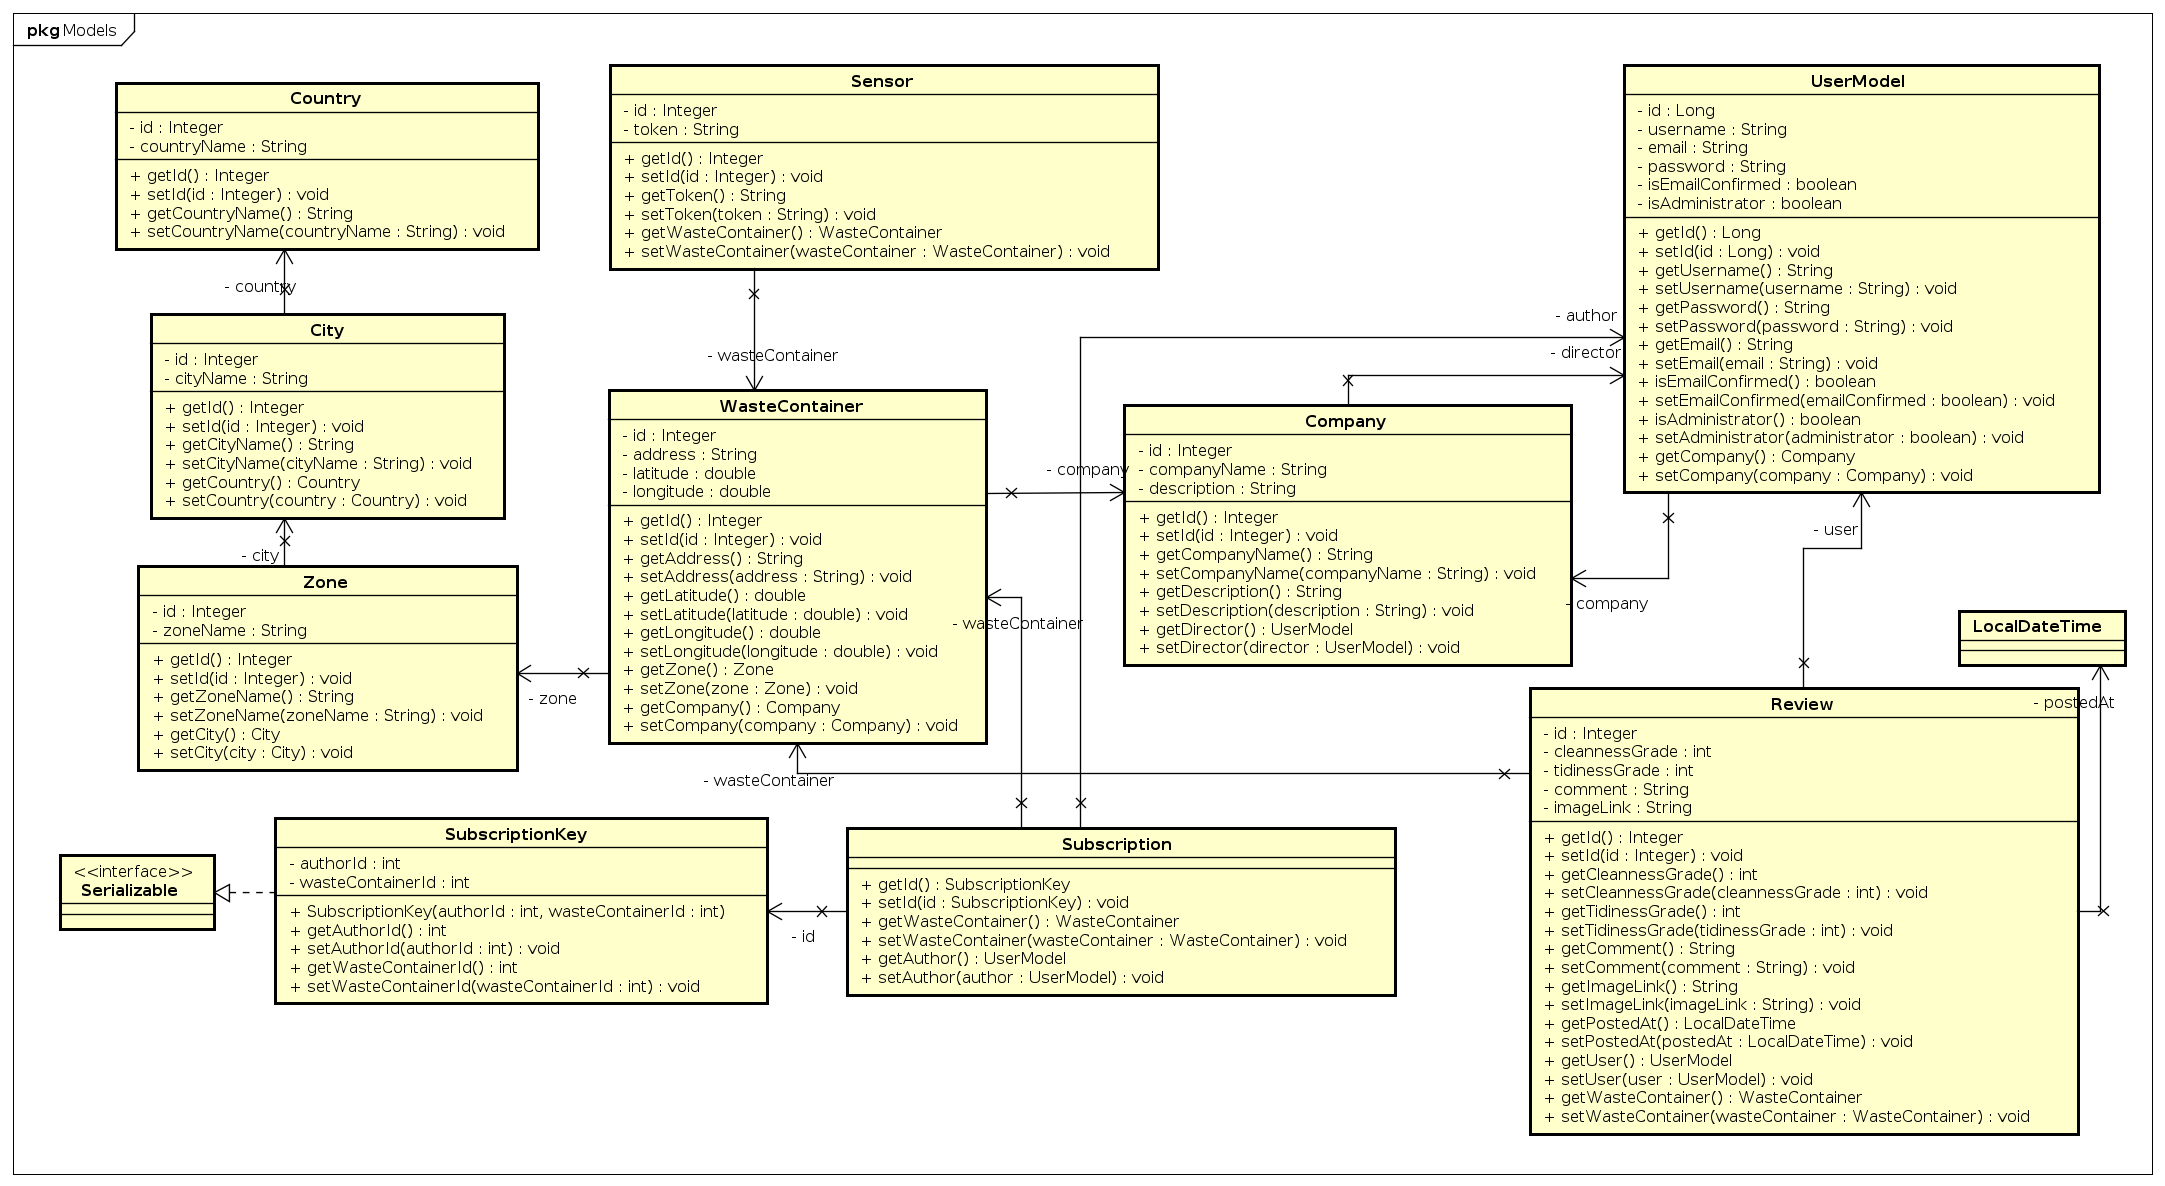
\includegraphics[width=1.0\linewidth]{slike/Models.png}
				\centering
				\caption{Dijagram razreda - dio Models}
				\label{fig:models}
			\end{figure}
		
%			\textbf{\textit{dio 2. revizije}}\\			
%			
%			\textit{Prilikom druge predaje projekta dijagram razreda i opisi moraju odgovarati stvarnom stanju implementacije}
			
			
			
			\eject
		
		\section{Dijagram stanja}
			
			
			Dijagram stanja prikazuje stanja objekta te prijelaze iz jednog stanja u drugo temeljene na događajima. Na slici 4.6 prikazan je dijagram stanja za registriranog korisnika - građanina. Nakon prijave, korisniku se prikazuje početna stranica na kojoj može pregledati kartu i kontejnere. Za odabrani kontejner ima opciju pregledavanja stanja (slika, komentara, ocjene urednosti), opciju za praćenje kontejnera te dodavanje vlastitog komentara, slike i ocjenjivanje kontejnera. Klikom na "Osobni podatci" prikazuju mu se njegovi podatci, koje može urediti ili odabrati opciju brisanja računa. Odabirom "Praćeni kontejneri" korisniku se otvara popis praćenih kontejnera koje po potrebi može obrisati.
			
			\begin{figure}[H]
				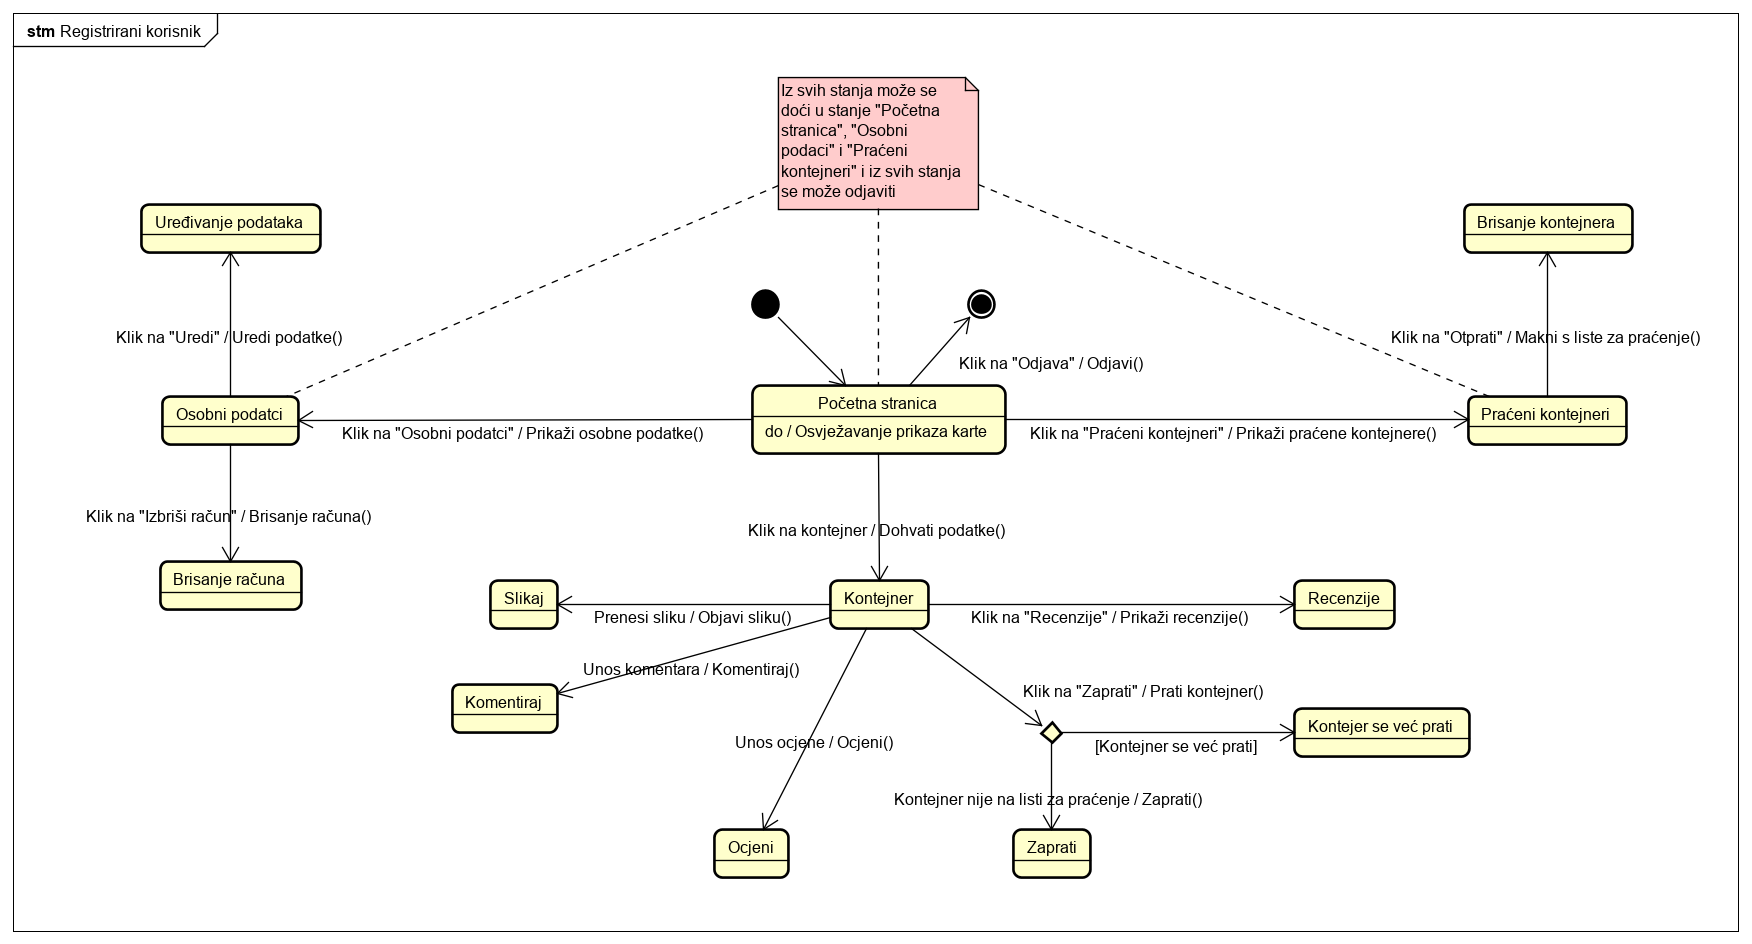
\includegraphics[width=1.0\linewidth]{slike/dijagramStanja.png}
				\centering
				\caption{Dijagram stanja}
				\label{fig:dijagramStanja}
			\end{figure}
			
			
			\eject 
		
		\section{Dijagram aktivnosti}
			
			Dijagram  aktivnosti  primjenjuje  se  za  opis  modela  toka  upravljanja  ili  toka  podataka.   Ne upotrebljava se za modeliranje događajima poticanog ponašanja. U modeliranju toka upravljanja svaki novi korak poduzima se nakon završenog prethodnog, a naglasak je na jednostavnosti.  Na dijagramu aktivnosti 4.7 prikazan je proces komentiranja stanja kontejnera. Korisnik se prijavi u sustav, odabere kontejner za koji želi ostaviti komentar, unese komentar. Kada je završio s pisanjem komentara, isti objavljuje te taj komentar postaje javan u recenzijama kontejnera.
			
			\begin{figure}[H]
				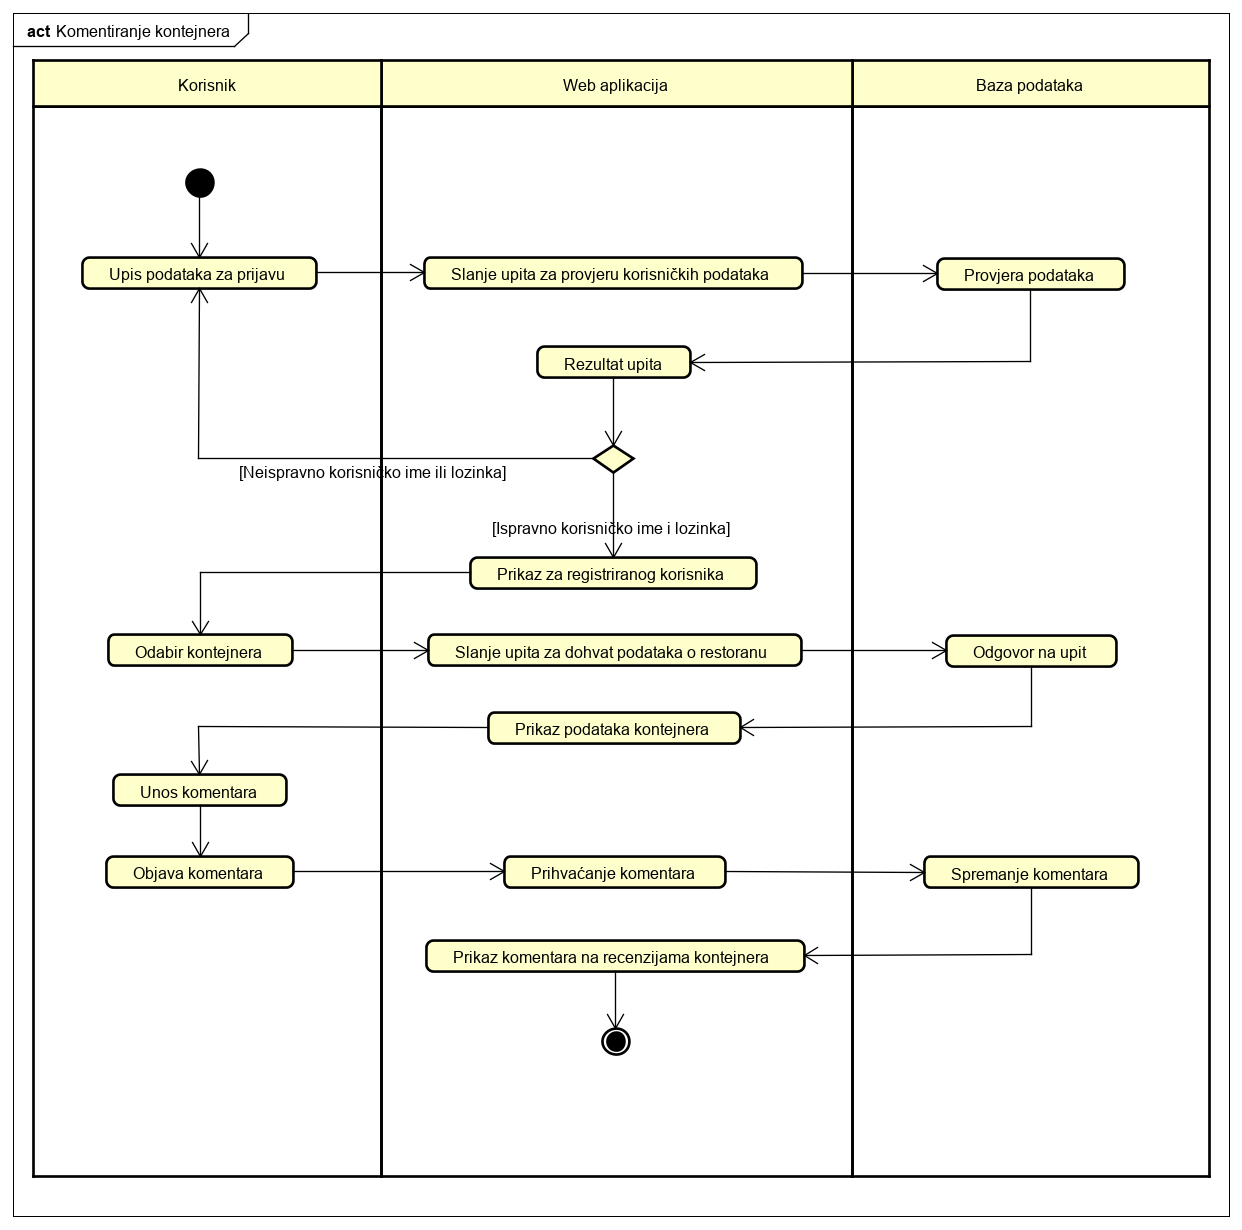
\includegraphics[width=1.0\linewidth]{slike/dijagramAktivnosti.png}
				\centering
				\caption{Dijagram aktivnosti}
				\label{fig:dijagramAktivnosti}
			\end{figure}
			
			\eject
		\section{Dijagram komponenti}
		
			Dijagram komponenti prikazan na sljedećoj stranici opisuje organizaciju i međuovisnost komponenti, interne strukture i odnose prema okolini. Sustavu se pristupa preko dva različita sučelja: sučelja za dohvat HTML, CSS i JS datoteka, preko kojega se poslužuju datoteke koje pripadaju \textit{frontend} dijelu aplikacije te sučelja za dohvat JSON podataka, preko kojega se pristupa REST API komponenti. Router je komponenta koja na upit s url određuje koja će se datoteka poslužiti na sučelje. \textit{Frontend} dio sastoji se od niza JavaScript datoteka koje su raspoređene u logičke cjeline nazvane po tipovima aktora koji im pristupaju. Sve JavaScript datoteke ovise o React biblioteci iz koje dohvaćaju gotove komponente (gumbe, forme, i sl.). REST API poslužuje podatke koji pripadaju \textit{backend} dijelu aplikacije. Hibernate je zadužen za dohvaćanje tablica iz baze podataka koristeći SQL upite. Ti podaci se dalje šalju MVC arhitekturi u obliku DTO (\textit{Data Transfer Object}) React-view komponenta komunicira preko dostupnih sučelja s Više Sreće Manje Smeće aplikacijom te osvježava prikaz i dohvaća nove podatke ili datoteke ovisno o korisnikovim akcijama.


			\eject

			\begin{figure}
				\centering
				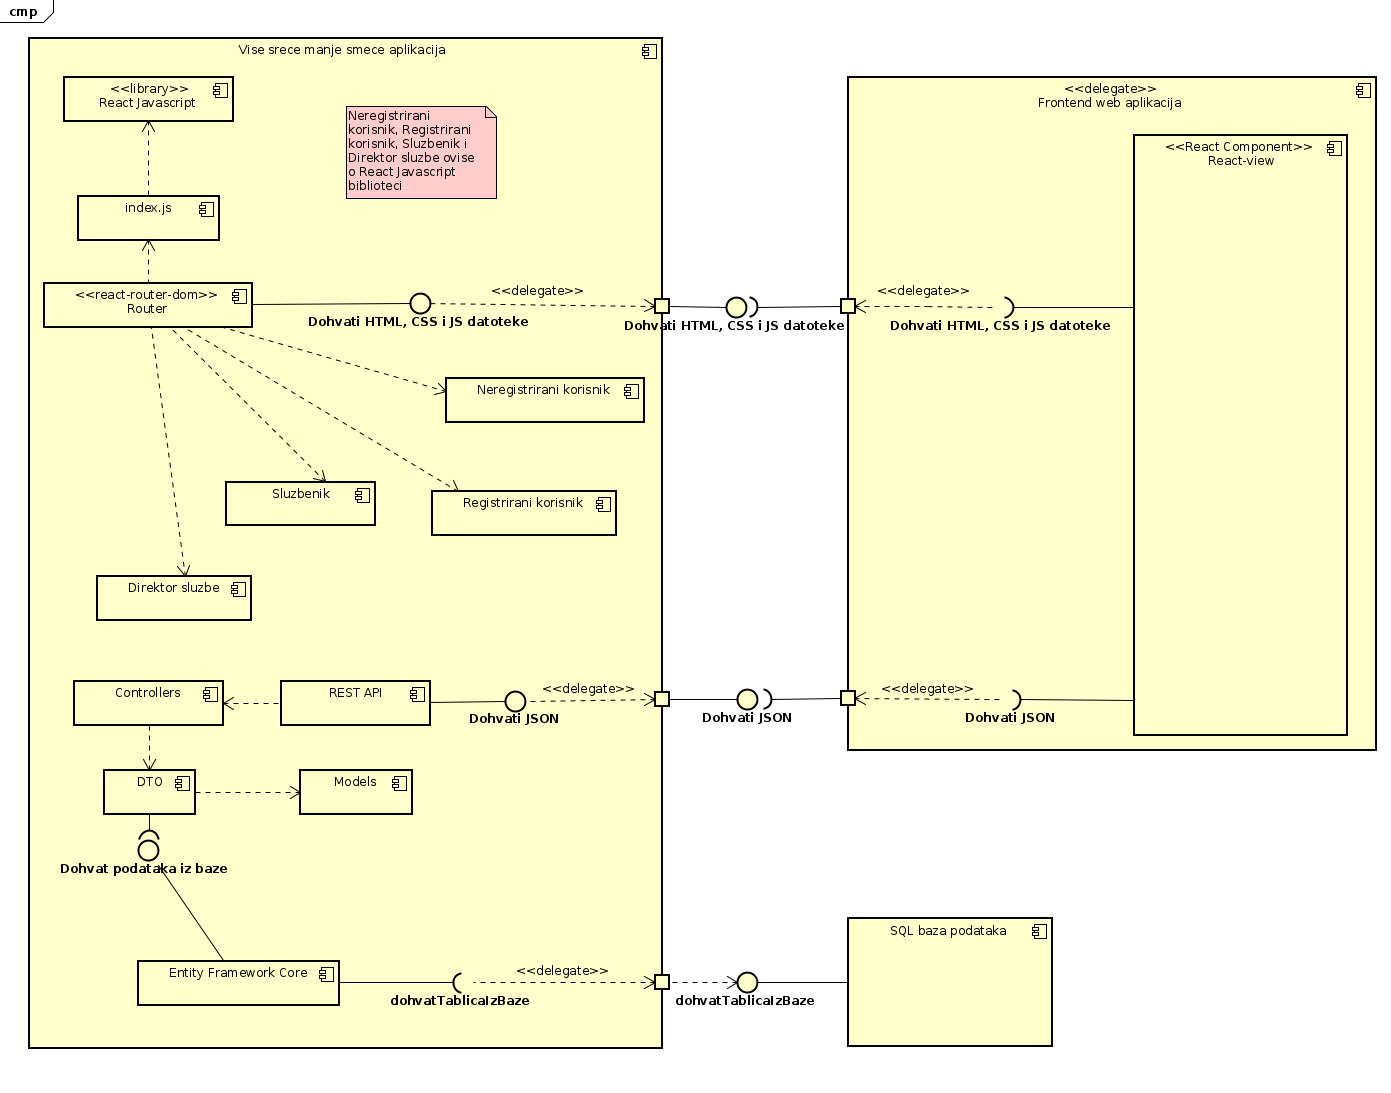
\includegraphics[width=1.0\linewidth]{slike/ComponentDiagram}
				\caption{Dijagram komponenti}
				\label{fig:ComponentDiagram}
			\end{figure}

			\clearpage
			\eject